% !TEX root = knottedMain.tex
\documentclass[varwidth=\maxdimen]{standalone}

\usepackage{mathtools,amssymb,mathrsfs,dutchcal,upgreek,faktor,accents,etoolbox,multicol}
\usepackage[dvipsnames]{xcolor}
\definecolor{mygreen}{RGB}{	8,156,79 }
\usepackage{tikz,tikz-cd}
\usetikzlibrary{patterns,knots,arrows.meta,decorations.markings}
\tikzset{>={Straight Barb[scale=0.85]}}
\tikzcdset{
  cells={font=\everymath\expandafter{\the\everymath\displaystyle}},
  arrow style=tikz,
  diagrams={>={Straight Barb[scale=0.85]}},
  every label/.append style = {font = \small}
}


\begin{document}
    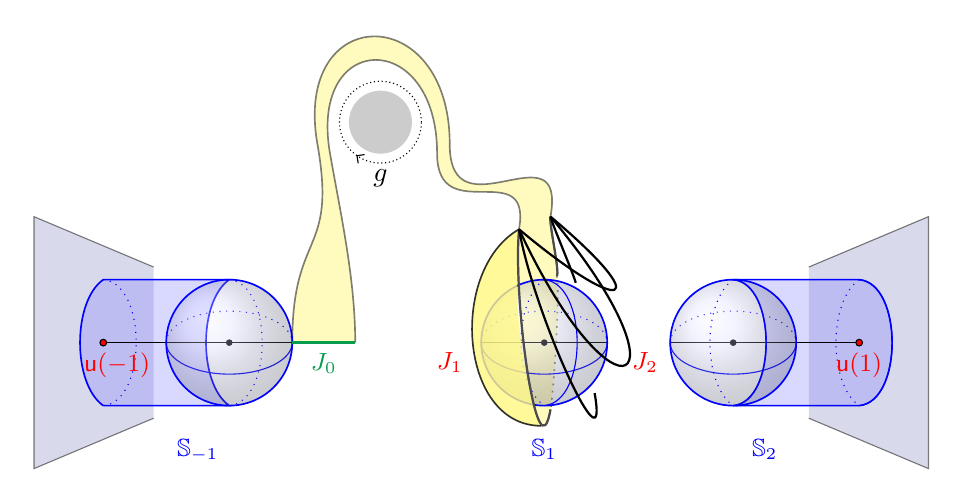
\begin{tikzpicture}[scale=0.8]
    \clip (-2.2,-2.1) rectangle (12.2,5);
% \begin{tikzpicture}[scale=0.7,every node/.style={scale=0.9},even odd rule,line width=0.2mm]
    % \clip (2.5,-1.33) rectangle (13.5,5.27);
    % BLACK HOLE
        \draw[thick, red]
        
        (4.5,0) node[below]{\small$J_{1}$}
        (7.6,0) node[below]{\small$J_{2}$}
        % (13.5,0) node[below]{$J_{4}$}
        % (16.5,0) node[below]{$J_{5}$}
        ;
    \fill[color=black!20!white] (3.4,3.5) circle (0.5cm);
    \draw[black,densely dotted,postaction=decorate,decoration = {markings, mark = at position 0.65 with {\arrowreversed{>}} }] (3.4,3.5) circle (0.65cm) node[below=0.48cm]{$g$};
    \fill[yellow!50,opacity=0.5]
                    (2,0) to[out=90, in=-80, distance=1.8cm]
                    (2.4,3.15) to[out=100, in=90, distance=2.3cm]
                    (4.5,3.15) to[out=-90, in=80, distance=1.5cm]
                    (6.1,2) to[in=40,out=-120, distance=0.07cm] 
                        (6.2,1.06)  to[out=-80, in=80, distance=0.3cm]
                        (6.1,-1.06)  to[in=-95,out=-100, distance=1.15cm]
                    (5.6,1.8) to[out=80,in=-90, distance=1.2cm] 
                    (4.3,3) to[in=100, out=90, distance=2cm]
                    (2.6,3) to[in=90, out=-80, distance=1cm]
                    (3,0) -- cycle ;
    \draw[black,semithick,opacity=0.5]
                    (2,0) to[out=90, in=-80, distance=1.8cm]
                    (2.4,3.15) to[out=100, in=90, distance=2.3cm]
                    (4.5,3.15) to[out=-90, in=80, distance=1.5cm]
                    (6.1,2) to[in=40,out=-120, distance=0.07cm] 
                        (6.2,1.06)  
                        (6.1,-1.06)  to[in=-95,out=-100, distance=1.15cm]
                    (5.6,1.8) to[out=80,in=-90, distance=1.2cm] 
                    (4.3,3) to[in=100, out=90, distance=2cm]
                    (2.6,3) to[in=90, out=-80, distance=1cm]
                    (3,0)  ;
    \draw[black,semithick,opacity=0.5,dotted]
        (6.2,1.06)  to[out=-80, in=80, distance=0.3cm]
                        (6.1,-1.06);

    % for crossings
    \fill[white] (8.2,-0.1) rectangle (9,0.1) ;
    % % sphere
    %     \shade[ball color=blue!5!white,opacity=0.6] (10,0) circle (1cm);
    %     \draw (10-1,0) arc (180:360:1cm and 0.5cm);
    %     \draw[dotted] (10-1,0) arc (180:0:1cm and 0.5cm);
    %     \draw (10,0) circle (1cm);




    % boundary of M
    \fill[blue!50!black,opacity=0.15,draw=black,draw opacity=0.5]
        (10.2,-1.2) -- (12.1,-2) -- (12.1,2) --  (10.2,1.2) ;
    \fill[blue!50!black,opacity=0.15,draw=black,draw opacity=0.5]
        (-0.2,1.2) -- (-2.1,2) -- (-2.1,-2) -- (-0.2,-1.2) ;
    % cylinder left
    \fill[draw=blue,semithick,fill=blue!50!white,fill opacity=0.3]
        (-1,-1) -- (1,-1) to[out=145,in=-145, distance=0.6cm] 
        (1,1) -- (-1,1) to[out=-145,in=145, distance=0.6cm] (-1,-1);
    \draw[semithick,blue] 
        (-1,1) -- (1,1) 
        (1,-1) -- (-1,-1);
    % vertical arcs on the first sphere
    \foreach \x in {-1,1}{
        % \draw[blue,semithick]
        %     (\x,1) to[out=-145,in=145, distance=0.6cm] (\x,-1);
        \draw[blue, dotted]
            (\x,1) to[out=-5,in=5, distance=0.7cm] (\x,-1);
    }
    % right cylinder
    \fill[draw=blue,semithick,fill=blue!50!white,fill opacity=0.3]
        (9,1) -- (11,1) to[out=-5,in=5, distance=0.7cm] 
        (11,-1) -- (9,-1) to[out=5,in=-5, distance=0.7cm] (9,1);
    % old
    \draw[semithick]
        (-1,0) -- (2,0)
        node[pos=0.5, below=1.1cm,blue]{\small$\mathbb{S}_{-1}$}
        (5,0) -- (7,0) node[pos=0.5, below=1.1cm,blue]{\small$\mathbb{S}_{1}$}
        (8,0) -- (11,0) node[pos=0.5, below=1.1cm,blue]{\small$\mathbb{S}_{2}$} ;

    % \draw[mygreen, thick]
    %     (0,0) -- (2,0) node[fill=mygreen!20,draw, pos=0.5]{}
    %     (1, 0) node[below=2pt]{$J_0$};
    \foreach \y/\ytext in {1/0,6/1,9/4}{
        \fill[fill=black] (\y,0) circle (1.5pt) 
        % node[below]{\small$u_{\ytext}$} 
        ;
    }
    %spheres
    \foreach \y in {1,6,9}{
        \draw[blue] (\y-1,0) arc (180:360:1cm and 0.5cm);
        \draw[blue,dotted] (\y-1,0) arc (180:0:1cm and 0.5cm);
        \shade[ball color=blue!20!,opacity=0.3] (\y,0) circle (1cm);
        \draw[blue,semithick] (\y,0) circle (1cm);
    }
    % vertical arcs
    \foreach \x in {6,9,11}{
        \draw[blue]
            (\x,1) to[out=-5,in=5, distance=0.7cm] (\x,-1);
        \draw[blue,dotted]
            (\x,1) to[out=-145,in=145, distance=0.6cm] (\x,-1);
    }
    % \foreach \y in {0,2}{
    %     \fill[mygreen,draw=black,semithick] (\y,0) circle (1.5pt);
    % }
    \fill[red,draw=black]
        (-1,0) circle (1.5pt) (-0.78,0) node[below]{\small$\mathsf{u}({-}1)$}
        (11,0) circle (1.5pt) node[below]{\small$\mathsf{u}(1)$};

    % yellow disk
    \fill[yellow!50!,opacity=0.8]
        (5.6,1.8) to[out=210,in=180, distance=1.3cm] (5.95,-1.32) to[in=-95,out=111, distance=1cm] (5.6,1.8) ;
    \draw[opacity=0.8,semithick]
        (5.6,1.8) to[out=210,in=180, distance=1.3cm] (5.95,-1.32)  ;


    % the yellow disk boundary
    \draw[black!70, thick]
                    (5.6,1.8) to[out=-95,in=-100, distance=1.15cm] (6.1,-1.06)
                    (6.2,1.06) to[out=40,in=-120, distance=0.07cm] (6.1,2) ;
    % the third from right
    \draw[,  thick]
            (5.6,1.8) to[out=-80,in=-80, distance=1.4cm] (6.8,-0.8)
            (6.5,0.95) to[out=100,in=-80, distance=0.1cm] (6.1,2) ;
    % the second from right
    \draw[,  thick]
           (5.6,1.8) to[out=-65,in=-50, distance=3.6cm] (6.1,2);
    % the rightmost
    \draw[,  thick]
            (5.6,1.8) to[out=-40,in=-40, distance=2.2cm] (6.1,2);
    
    \draw[mygreen, very thick]
        (2,0) -- (3,0)  node[pos=0.5,below]{\small$J_0$};
\end{tikzpicture}

\end{document}
